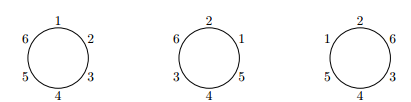
\includegraphics{birthday.png}

Левая картинка показывает начальное расположение детей. Средняя --- результат следующей пересадки: дети с номерами 1 и 2 двигаются на одну поизицию, дети с номерами 3 и 5 на две, и дети с номерами 4 и 6 не меняют свою позицию. Условия рассадки соблюдены, так как 3 места находятся между 6 и 4, 4 места между 3 и 5, 5 мест между 4 и 1, 1 место между 5 и 2, 2 места между 1 и
6, и 6 мест между 2 и 3. Существует и другой способ рассадки, указанный на правой картинка. В обоих случаях никто из детей не двигается больше чем на два места.
